\par\clearpage
\normalmarginpar
\scanpage{4}
\noindent\margin{\vspace*{5.3\baselineskip}SGA 7}\par

% The two long pen strokes, including their returns at the bottom, cross several rows.
\begingroup
\small
\setlength{\arraycolsep}{3pt}
\renewcommand{\arraystretch}{2.05}
\diagram{\figure{\resizebox{\linewidth}{!}{%
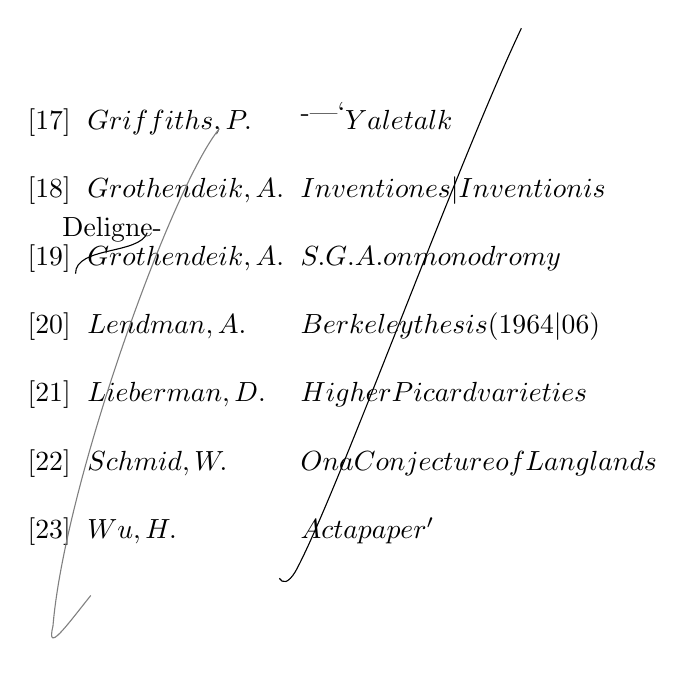
\begin{tikzpicture}
\node[anchor=south west,inner sep=0pt] (refs) at (0,0) {%
$\begin{array}{@{}lll@{}}
\text{[17]}&\text{Griffiths, P.}&\text{\raisebox{.6ex}{\unsure{-|\textquoteleft}}Yale talk}\\
\text{[18]}&\text{Grothendeik, A.}&\text{\unsure{Inventiones|Inventionis}}\\
\text{[19]}&\text{\rlap{\hspace*{-.9em}\raisebox{1.05em}{\inserted{Deligne-}}}\tikz[baseline,overlay]{\draw (-.15,-.10) .. controls (-.15,.25) and (.66,.14) .. (.76,.42);}Grothendeik, A.}&\text{S.G.A. on monodromy}\\
\text{[20]}&\text{Lendman, A.}&\text{Berkeley thesis (196\deleted{\unsure{4|0}}6)}\\
\text{[21]}&\text{Lieberman, D.}&\text{Higher Picard varieties}\\
\text{[22]}&\text{Schmid, W.}&\text{On a Conjecture of Langlands}\\
\text{[23]}&\text{Wu, H.}&\text{Acta paper\textquoteright}
\end{array}$};
\begin{scope}[x={(refs.south east)},y={(refs.north west)}]
\draw[gray] (.305,.90) .. controls (.23,.78) and (.06,.16) .. (.041,-.14)
    .. controls (.030,-.20) and (.062,-.14) .. (.101,-.076);
\draw (.784,1.11) .. controls (.68,.82) and (.49,.13) .. (.426,-.025)
    .. controls (.414,-.052) and (.405,-.051) .. (.400,-.040);
\end{scope}
\end{tikzpicture}}}}
\endgroup

% archive sheet number: 3
